


\captionsetup[subfigure]{font=scriptsize}
\begin{figure}[t]
%\centering
\begin{subfigure}{0.57\linewidth}
% %\centering
\begin{tikzpicture}
\begin{groupplot}[
    group style={
        group size=1 by 2,
        vertical sep=0.4cm, % Gap between the two plots
        x descriptions at=edge bottom, % Only show x labels on bottom plot
    },
    width=1.25\linewidth,
    symbolic x coords={LLM,OA,AG,LG,CA,Ag,OS,Co},
    xtick=data,
    ybar,
    % bar width=3pt,
    /pgf/bar width=3pt,
    enlarge x limits=0.15,
    ymajorgrids=true,
    grid style={dashed,gray!30},
    tick label style={font=\tiny},
    ylabel style={font=\tiny},
    xlabel style={font=\tiny},
    every axis plot/.append style={fill opacity=0.9},
    nodes near coords,
    nodes near coords style={
        font=\tiny, yshift=7pt, xshift=5pt, anchor=south, rotate=90
    }
]

% --- TOP PLOT (Outlier Range) ---
\nextgroupplot[
    height=2.5cm,
    ymin=44, ymax=70, % Range for Concordia
    ytick={40, 50, 60},
    axis x line*=top
, % Hide the x-axis for the top part
    legend style={
        at={(0.02,0.98)},
        anchor=north west,
        font=\tiny,
        legend columns=-1
    },
    ylabel={Latency (s)},
    ylabel style={at={(axis description cs:1.03, -1.2)}, anchor=west}, % Centered label
]
\addplot+[fill=blue!60] coordinates {
    (LLM,0.379) (OA,0.495) (AG,0.496) (LG,0.524)
    (CA,0.611) (Ag,0.860) (OS,1.170) (Co,44.473)
};
\addplot+[fill=green!60] coordinates {
    (LLM,0.730) (OA,0.840) (AG,0.787) (LG,1.093)
    (CA,0.801) (Ag,1.183) (OS,2.036) (Co,53.420)
};
\legend{p50, p95}

% --- BOTTOM PLOT (Main Data Range) ---
\nextgroupplot[
    height=2.3cm,
    ymin=0, ymax=3, % Range for all other agents
    ytick={0, 1, 2, 3},
    axis x line*=bottom,
    xticklabel style={rotate=90, anchor=east, font=\tiny},
    % axis y discontinuity=parallel, % Adds the visual "break" symbol
]
\addplot+[fill=blue!60] coordinates {
    (LLM,0.379) (OA,0.495) (AG,0.496) (LG,0.524)
    (CA,0.611) (Ag,0.860) (OS,1.170) (Co,44.473)
};
\addplot+[fill=green!60] coordinates {
    (LLM,0.730) (OA,0.840) (AG,0.787) (LG,1.093)
    (CA,0.801) (Ag,1.183) (OS,2.036) (Co,53.420)
};

\end{groupplot}
\end{tikzpicture}
\vspace{-7mm}
\caption{Latency}
\end{subfigure}
% \hspace{1mm}
% \hfill
% ---------------- Throughput ----------------
\begin{subfigure}{0.42\linewidth}
%\centering
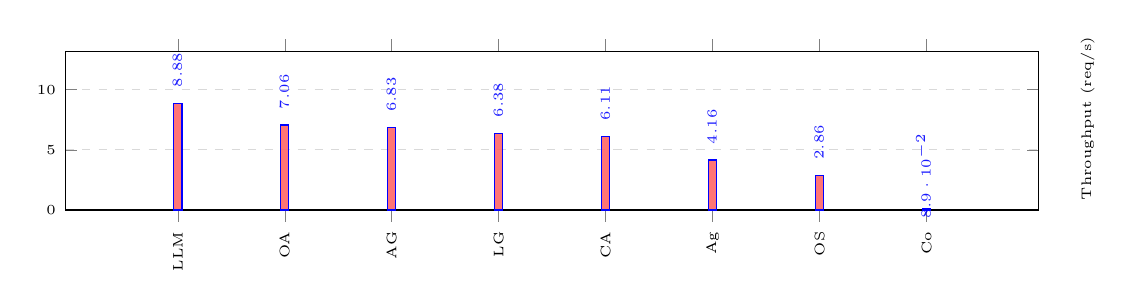
\begin{tikzpicture}
\begin{axis}[
    width=1.15\linewidth,
    height=3.6cm,
    ymin=0,
    ymax=13.206,
    % symbolic x coords={Direct LLM,OpenAgents,AutoGen,LangGraph,CrewAI,Agno,OpenAISDK,Concordia},
    symbolic x coords={ LLM,OA,AG,LG,CA,Ag,OS,Co},
    xtick=data,
    xticklabel style={rotate=90, anchor=east, font=\tiny},
    ylabel={Throughput (req/s)},
    ylabel style={at={(axis description cs:1.05,0.)}, anchor=west},
    tick label style={font=\tiny},
    ylabel style={font=\tiny},
    xlabel style={font=\tiny},
    ybar,
    bar width=3pt,
    enlarge x limits=0.15,
    ymajorgrids=true,
    grid style={dashed,gray!30},
    nodes near coords,
    nodes near coords style={
        font=\tiny,
        yshift=12pt,
        xshift=5pt,
        anchor=south,
        rotate=90
    },
    every axis plot/.append style={fill opacity=0.9},
]
% \addplot+[fill=red!60] coordinates {(Direct LLM,8.875) (OpenAgents,7.062) (AutoGen,6.827) (LangGraph,6.377) (CrewAI,6.113) (Agno,4.158) (OpenAISDK,2.860) (Concordia,0.089)};
\addplot+[fill=red!60] coordinates {(LLM,8.875) (OA,7.062) (AG,6.827) (LG,6.377) (CA,6.113) (Ag,4.158) (OS,2.860) (Co,0.089)};
\end{axis}
\end{tikzpicture}
\vspace{-3mm}
\caption{Throughput}
\end{subfigure}


\hspace{-2mm}
% ---------------- Mean Output ---------------- 
\begin{subfigure}{0.42\linewidth}
%\centering
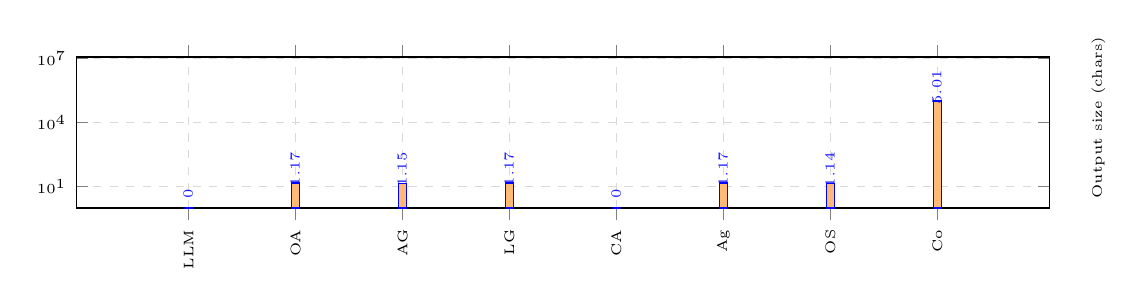
\begin{tikzpicture}
\begin{semilogyaxis}[
    width=1.15\linewidth,
    height=3.5cm,
    ymode=log,
    log basis y=10,
    ymin=1,
    ymax=11799100.564,
    % symbolic x coords={Direct LLM,OpenAgents,AutoGen,LangGraph,CrewAI,Agno,OpenAISDK,Concordia},
    symbolic x coords={ LLM,OA,AG,LG,CA,Ag,OS,Co},
    xtick=data,
    grid=major,
    xticklabel style={rotate=90, anchor=east, font=\tiny},
    ylabel={Output size (chars)},
    ylabel style={at={(axis description cs:1.05,0.)}, anchor=west},
    tick label style={font=\tiny},
    ymajorgrids=true,
    grid style=dashed,
    ylabel style={font=\tiny},
    xlabel style={font=\tiny},
    ybar,
    bar width=3pt,
    enlarge x limits=0.15,
    ymajorgrids=true,
    grid style={dashed,gray!30},
    nodes near coords,
    nodes near coords style={
        font=\tiny,
        yshift=5pt,
        xshift=5pt,
        anchor=south,
        rotate=90
    },
    every axis plot/.append style={fill opacity=0.9}
]
% \addplot+[fill=orange!60] coordinates {(Direct LLM,1.000) (OpenAgents,14.900) (AutoGen,14.220) (LangGraph,14.900) (CrewAI,1.000) (Agno,14.800) (OpenAISDK,13.880) (Concordia,102601.360)};
\addplot+[fill=orange!60] coordinates {
    (LLM,1.000) (OA,14.900) (AG,14.220) (LG,14.900)
    (CA,1.000) (Ag,14.800) (OS,13.880) (Co,102601.360)
};

\end{semilogyaxis}
\end{tikzpicture}
\vspace{-3mm}
\caption{Mean output}
\end{subfigure}
% ---------------- Output Summary ----------------
\hspace{-4mm} 
\begin{subfigure}{0.57\linewidth}
%\centering
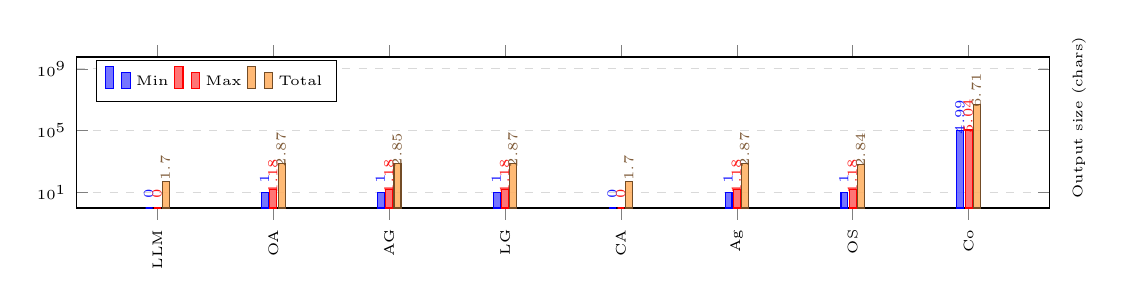
\begin{tikzpicture}
\begin{axis}[
    width=1.15\linewidth,
    height=3.5cm,
    ymode=log,
    log basis y=10,
    ymin=1,
    ymax=5899578000.200,
    % symbolic x coords={Direct LLM,OpenAgents,AutoGen,LangGraph,CrewAI,Agno,OpenAISDK,Concordia},
    symbolic x coords={ LLM,OA,AG,LG,CA,Ag,OS,Co},
    xtick=data,
    xticklabel style={rotate=90, anchor=east, font=\tiny},
    ylabel={Output size (chars)},
    ylabel style={at={(axis description cs:1.03,0.)}, anchor=west},
    legend style={
    at={(0.02,0.98)},
    anchor=north west,
    font=\tiny,
    legend columns=-1
    },
    tick label style={font=\tiny},
    ylabel style={font=\tiny},
    xlabel style={font=\tiny},
    ybar,
    bar width=2.5pt,
    enlarge x limits=0.1,
    ymajorgrids=true,
    grid style={dashed,gray!30},
    nodes near coords,
    nodes near coords style={
        font=\tiny,
        yshift=5pt,
        xshift=5pt,
        anchor=south,
        rotate=90
    },
    every axis plot/.append style={fill opacity=0.9}
]
% \addplot+[fill=blue!60] coordinates {(Direct LLM,1.000) (OpenAgents,10.000) (AutoGen,10.000) (LangGraph,10.000) (CrewAI,1.000) (Agno,10.000) (OpenAISDK,10.000) (Concordia,97448.000)};
% \addplot+[fill=red!60] coordinates {(Direct LLM,1.000) (OpenAgents,15.000) (AutoGen,15.000) (LangGraph,15.000) (CrewAI,1.000) (Agno,15.000) (OpenAISDK,15.000) (Concordia,110886.000)};
% \addplot+[fill=orange!60] coordinates {(Direct LLM,50.000) (OpenAgents,745.000) (AutoGen,711.000) (LangGraph,745.000) (CrewAI,50.000) (Agno,740.000) (OpenAISDK,694.000) (Concordia,5130068.000)};
\addplot+[fill=blue!60, bar shift=-3pt] coordinates {
    (LLM,1.000) (OA,10.000) (AG,10.000) (LG,10.000)
    (CA,1.000) (Ag,10.000) (OS,10.000) (Co,97448.000)
};

\addplot+[fill=red!60, bar shift=-0pt] coordinates {
    (LLM,1.000) (OA,15.000) (AG,15.000) (LG,15.000)
    (CA,1.000) (Ag,15.000) (OS,15.000) (Co,110886.000)
};

\addplot+[fill=orange!60, bar shift=3pt] coordinates {
    (LLM,50.000) (OA,745.000) (AG,711.000) (LG,745.000)
    (CA,50.000) (Ag,740.000) (OS,694.000) (Co,5130068.000)
};

\legend{Min, Max, Total}
\end{axis}
\end{tikzpicture}
\vspace{-7mm}
\caption{Output summary}
\end{subfigure}
\hfill
\vspace{0mm}
\noindent\fbox{%
  \parbox{0.85\linewidth}{\scriptsize
  \textbf{Abbreviations:}
  LLM=Direct LLM;
  OA=OpenAgents;
  AG=AutoGen;
  LG=LangGraph; \\
  CA=CrewAI;
  Ag=Agno;
  OS=OpenAI SDK;
  Co=Concordia.
  }
}
\vspace{-4mm}
\caption{
Framework overhead on a trivial task (“What is 2+2?”) over 50 trials.
Frameworks are ordered by p50 latency.
}
\vspace{-4mm}
\label{fig:framework-overhead}
\end{figure}



